\documentclass{article}
\usepackage[T1]{fontenc}
\usepackage{lmodern}
\usepackage{graphicx}
\usepackage{amsmath,amssymb}
\usepackage[a4paper,margin=2cm]{geometry}
\usepackage[absolute,overlay]{textpos}
\setlength{\TPHorizModule}{1mm}
\setlength{\TPVertModule}{1mm}
\usepackage[indonesian]{babel}
\usepackage{hyperref}
\setlength{\emergencystretch}{2em}
% unit: Halaman 37

\begin{document}

% === Halaman 37 (llm) ===

Sebagai contoh, misalkan $key$ dalam hekadesimal adalah

\[ key = (54, 77, 6F, 20, 4F, 6E, 65, 20, 4E, 69, 6E, 65, 20, 54, 77, 6F) \]

\vspace{63.26mm}

Dari $key$ langsung diperoleh $rk[0]$ sebagai berikut:

\vspace{5mm}

% deskripsi: Tabel matriks yang berisi nilai heksadesimal hasil pemetaan dari kunci (key) menjadi rk[0].
% bbox normalisasi: [0.2820, 0.4520, 0.4910, 0.6650]
\begin{textblock*}{43.89mm}(59.22mm,134.24mm)
\noindent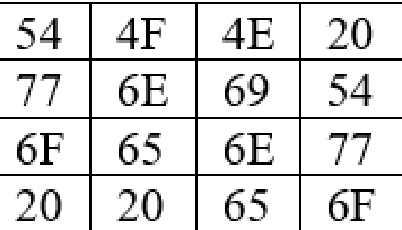
\includegraphics[width=43.89mm,height=63.26mm]{../../images/llm/page_037_img_01.png}%
\end{textblock*}

\end{document}
